\section{R2U2 Software Implementation in C++}
The C++ version of R2U2 can be executed offline, as a trace and/or MLTL formula validation tool, or online, as a streaming runtime monitor. The offline version serves as a way for a user to validate an MLTL formula over a trace and it helps developer's perform regression testing across pre-validated traces \& formulae. The online version executes a streaming runtime monitor, which can execute on either an embedded processor or a personal computer. Similar to the R2U2-C version, the embedded sensor's data must be saved into a file structure that R2U2 accesses. Additionally, the sensor data must be pre-processed into Boolean atomics before R2U2-C++ can reason over them.

\subsection{Getting Started}
The C++ implementation of R2U2 runs from a UNIX based command line interface (CLI). Additionally, there are several types of files users must use:
\begin{itemize}
	\item \textbf{Assembly File:} The \textit{.ftasm} file that stores the assembly code for the MLTL formula. The details and an example of this 
	\item \textbf{Trace File:} The sensor information from either an offline or online trace need to be stored into one or more \textit{.log} files. The details for how to modify the \textit{MTL.cpp} file for the user specific \textit{.log} files, how to format the \textit{.log} files, and examples of each will be given in Section \ref{Cpp_Sensor}.
	\end{itemize}
	

\subsection{File Formats}
Note that user must provide the \textit{.ftasm} file and one or more \textit{.log} files to run this version of R2U2. The \textit{.ftasm} assembly file specifies the temporal logic formulas over which the atomic propositions are reasoned over. The \textit{.log} files are the atomic sensor traces that are being reasoned over.

\subsubsection{Assembly File:}
\label{AssemblyFile}
Like any other assembly file, this file is a list of single command instructions that R2U2 will execute, in order. An example of a R2U2 compatible Assembly File can be seen in Table \ref{CppFileTable}. Each line contains an instruction, which consists of a label, a command, and one or more variables/labels. The list of assembly commands the C++ version of R2U2 can use is:
\begin{itemize}
	\item \textbf{\textit{load}:} Used to load the atomic from either the Sensor Input File or Atomic Input File. 
	\item \textbf{\textit{not}:} Used to denote the logical \textit{Negation} of an atomic.
	\item \textbf{\textit{and}:} Used to denote the logical \textit{AND} of two atomics.
	\item \textbf{\textit{until}:} Used to denote the \textit{Until} temporal logic function. This function takes in four arguments: the first is the label for the left-side of the \textit{Until}, the second is the right-side, the third is the relative start time, and the fourth is the relative end time.
	\item \textbf{\textit{boxbox}:} Used to denote the \textit{Global} temporal logic function. Assumes that the time bound starts at zero. First argument is the label (either atomic or instruction), the second is the relative end time of the function.
	\item \textbf{\textit{boxdot}:} Used to denote the \textit{Global} temporal logic function. First argument is the label (either atomic or instruction), the second is the relative start time of the function, and the third is the relative end time of the function.
	\item \textbf{\textit{end}:} Used to denote the end of the assembly file. This command must be at the end of the Assembly File and its argument must be the second-to-last label.
\end{itemize}

\begin{table}[H]
	\caption{Examples of the format for the \textit{.ftasm} file.
	\label{CppFileTable}}
	\begin{center}
	\begin{tabular}{l | l}
		\hline
		\hline
		\textbf{File Type} & \textbf{Assembly File}\\
		\hline
		line 1 & load\_ft a000\\
		line 2 & load\_ft a001\\
		line 3 & not s000\\
		line 4 & not s001\\
		line 5 & and s002 s003\\
		line 6 & and s000 s001\\
		line 7 & not s005\\
		line 8 & until s006 s005 0 3\\
		line 9 & boxbox s007 3\\
		line 10 & end s008\\
		\hline
		\hline
	\end{tabular}
	\end{center}
\end{table}

\subsubsection{Trace File Formats}
\label{Cpp_Sensor}
The trace information must be passed to R2U2-C++ via \textit{.log} files. These \textit{.log} files must be specified in the \textit{MTL.cpp} file. How this is done as well as the formatting for the input files will be described in this section.

\subparagraph{Modifying the \textit{MTL.cpp}}
\label{Mod_MTL}
Within the \textbf{R2U2\_SW/R2U2\_Cpp/src} directory is the \textit{MTL.cpp} file. This file must be modified in order to interface R2U2 with all of the \textit{.log} files R2U2 will read. A screenshot of the code that must be modified can be seen in Fig. \ref{fig:r2u2cppMod}. 

\begin{figure}[H]
	\begin{center}
	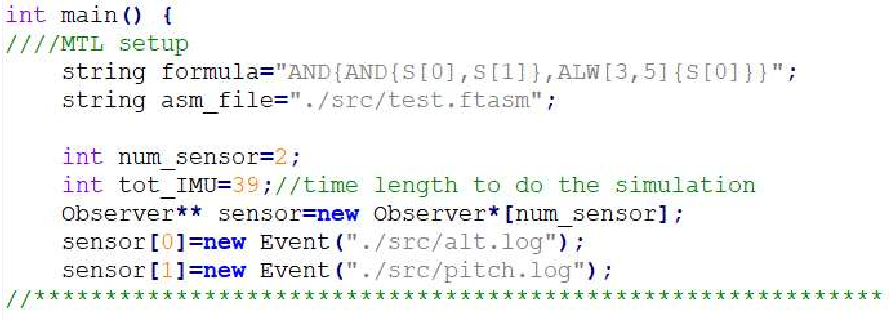
\includegraphics[scale=0.5]{fig/r2u2_cpp_MTL.pdf}
	\caption{A screenshot of the user modified code in \textit{MTL.cpp}. In this example, there are two sensor traces: \textit{alt.log} and \textit{pitch.log}.
	\label{fig:r2u2cppMod}} 
	\end{center}
\end{figure} 

Several values must be tailored to the specific project, namely: \textbf{num\_sensor} and \textbf{tot\_IMU} must be set to the specific number of \textit{.log} files for the application as well as how many time stamps long R2U2 will execute. For each \textit{.log} file, the \textit{.log} file's location must be specified within the \textbf{sensor} array.

\subparagraph{Atomic Input File:}
\label{Cpp_InputFile}
The values of the atomic input file must be Booleans, i.e., a $0$ or $1$. Thus, the sensor value must be pre-processed into a Boolean value via a comparison operator. An example of the format can be seen in Table \ref{CppTraceTable}.

\begin{table}[H]
	\caption{Examples of the format for the Trace Files.
	\label{CppTraceTable}}
	\begin{center}
	\begin{tabular}{l | cc}
		\hline
		\hline
		\textbf{File Type} & \multicolumn{2}{c}{\textbf{Atomic Input File}}\\
		\hline
		Line \# & Atomic & Time\\
		\hline
		line 1 & 0 & 0\\
		line 2 & 0 & 1\\
		line 3 & 1 & 2\\
		line 4 & 0 & 3\\
		line 5 & 1 & 4\\
		$\vdots$ & $\vdots$ & $\vdots$\\
		\hline
		\hline
	\end{tabular}
	\end{center}
\end{table}

\subsection{CLI Overview}
\begin{enumerate}
%***** #1	
	\item Navigate to the \textbf{R2U2\_SW/R2U2\_Cpp/src} directory via:
	\begin{lstlisting}[language=C]
	cd R2U2_Cpp/src
	\end{lstlisting}
	\begin{enumerate}
	%***** #a
		\item For the offline version of R2U2-C++, place the sensor trace files in this directory, following the syntax from Section \ref{Cpp_InputFile}.
		\item For the online version of R2U2-C++, ?
	\end{enumerate}
%***** #2
	\item Modify \textit{MTL.cpp} sensor input information. The quantity of sensors and the files the sensor information will be read from must be modified. See Section \ref{Cpp_Sensor} for details.
%***** #3
	\item Navigate to the \textbf{R2U2\_SW/R2U2\_Cpp} directory via:
	\begin{lstlisting}[language=C]
	cd ../
	\end{lstlisting}
%***** #4
	\item Compile R2U2-C++ via:
	\begin{lstlisting}[language=C]
	make
	\end{lstlisting}
%***** #5
	\item To launch R2U2-C++, exectute:
	\begin{lstlisting}[language=C]
	./build/app/main
	\end{lstlisting}
\end{enumerate}

\clearpage
